\documentclass[11pt]{article}

\usepackage[margin=0.85in]{geometry}
\usepackage{amsmath,amssymb}
\usepackage{booktabs}
\usepackage{graphicx}
\usepackage{pdfpages}
\usepackage{microtype}
\usepackage{parskip}
\usepackage{float}
\usepackage[font=small,labelfont=bf]{caption}
\usepackage[colorlinks=true,linkcolor=blue!55!black,urlcolor=blue!55!black]{hyperref}
\usepackage{xcolor}

\graphicspath{{figures/}}
\newcommand{\Bchord}{B_{\mathrm{chord}}}
\newcommand{\Bworse}{B_{\mathrm{worse}}}

\title{Training-Stage Connectivity in VGG11 on CIFAR-10\\
\large Experimental results and interpretation}
\author{M. P. Lodzinski}
\date{28 September 2026}

\begin{document}
\maketitle

\begin{abstract}
This report asks how compatibility between independently trained networks
changes during training.  Three pairs of VGG11 models are compared at twelve
checkpoints using symmetry-aligned linear interpolation and optimized nonlinear
paths.  Linear incompatibility appears within the first few epochs, permutation
alone leaves large barriers, and positive scaling removes most of the
remaining worse-endpoint barrier.  Optimized B\'ezier and polygonal paths remove
more than 99\% of the raw test-loss chord barrier on average.  The conclusions
are empirical statements about the tested alignment algorithms and path
families, rather than claims about all possible transformations or paths.
\end{abstract}

\section{Question and experimental idea}

Standard mode-connectivity studies compare converged solutions.  Here we ask
when two independent runs become incompatible.  Since an early checkpoint is
not necessarily a local minimum, we call this \emph{training-stage
connectivity}.  For checkpoints $\theta_A^{(n)}$ and $\theta_B^{(m)}$, we study:

\begin{itemize}
    \item same-stage pairs $A_n$--$B_n$;
    \item cross-stage pairs $A_{200}$--$B_n$ and $A_n$--$B_{200}$;
    \item within-run controls $A_n$--$A_{200}$ and $B_n$--$B_{200}$.
\end{itemize}

Six independently trained no-BN VGG11 models are grouped into three seed
pairs.  We use epochs
$\{0,1,2,3,5,10,20,30,60,100,150,200\}$, treating epoch zero as an
initialization control.

The linear experiment compares raw interpolation, weight matching, Sinkhorn,
and positive-scaling extensions of both alignment families.  Validation data
select the best permutation-only method and the best method overall for each
ordered checkpoint pair.  These choices are then frozen and evaluated on two
additional seed pairs.

The nonlinear experiment keeps the raw endpoints fixed.  A quadratic B\'ezier
path is fitted for every same-stage, cross-stage, and within-run pair.  Difficult
pairs receive additional B\'ezier and two-bend polygonal restarts.  Validation
data select the final path before test evaluation.

\section{Two complementary barrier definitions}

For a path $\gamma(\lambda)$ with endpoint costs $C(\theta_A)$ and
$C(\theta_B)$, the conventional chord barrier is
\begin{equation}
\Bchord=\sup_{\lambda\in[0,1]}
\left[C(\gamma(\lambda))-\left((1-\lambda)C(\theta_A)
+\lambda C(\theta_B)\right)\right].
\label{eq:chord}
\end{equation}
It measures the largest deviation above the line joining the endpoint costs.
We also report
\begin{equation}
\Bworse=\sup_{\lambda\in[0,1]}C(\gamma(\lambda))
-\max\{C(\theta_A),C(\theta_B)\},
\label{eq:worse}
\end{equation}
which asks whether the path becomes worse than the worse endpoint.

\begin{figure}[H]
    \centering
    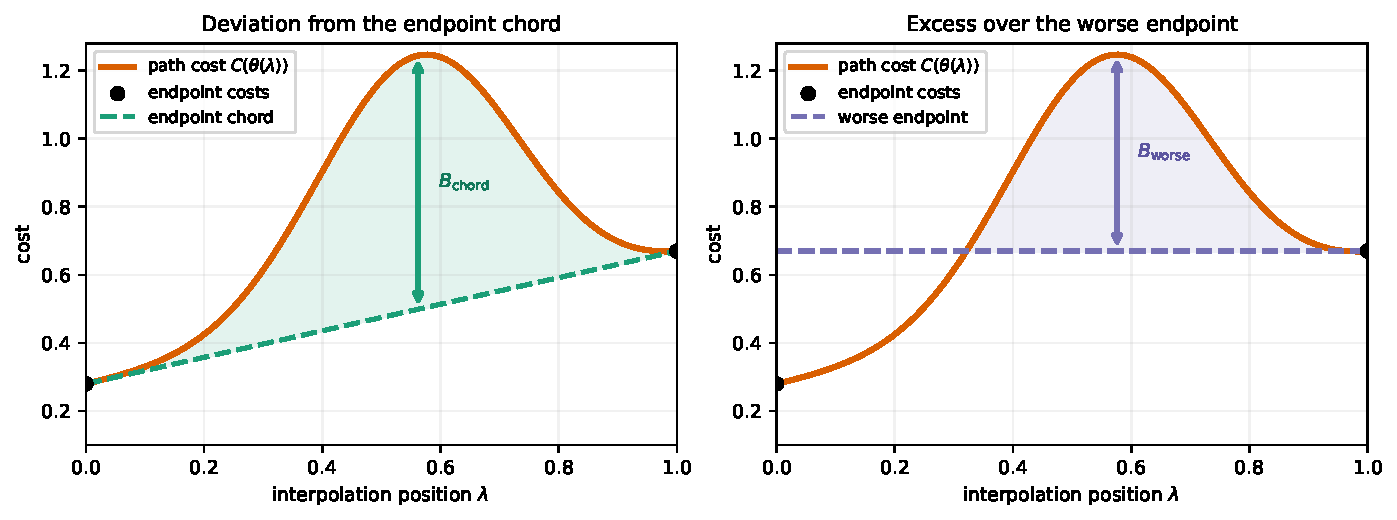
\includegraphics[width=0.95\linewidth]{barrier_definitions.pdf}
    \caption{The same path evaluated by $\Bchord$ and $\Bworse$.  The
    distinction matters most when the endpoint losses are unequal.}
    \label{fig:barriers}
\end{figure}

Both quantities are needed.  For example, a random early endpoint can make
$\Bworse$ zero simply because it already has high loss, while $\Bchord$ still
detects curvature above the endpoint trend.  Conversely, $\Bchord$ does not
directly answer whether the path is worse than either endpoint.  Both metrics
are sampled estimates and should be interpreted together with absolute loss.

\section{Linear stage connectivity}

\subsection{Same-stage results}

Figure~\ref{fig:linear-same} compares the best permutation-only method with
the best overall method, which may use positive scaling.  A large
permutation-only barrier appears almost immediately: mean test-loss
$\Bworse$ is $0.375$ after one epoch and peaks at $0.834$ at epoch 5.  It then
declines to $0.251$ at epoch 200.  Linear incompatibility therefore develops
early and is not monotonic throughout training.

\begin{figure}[H]
    \centering
    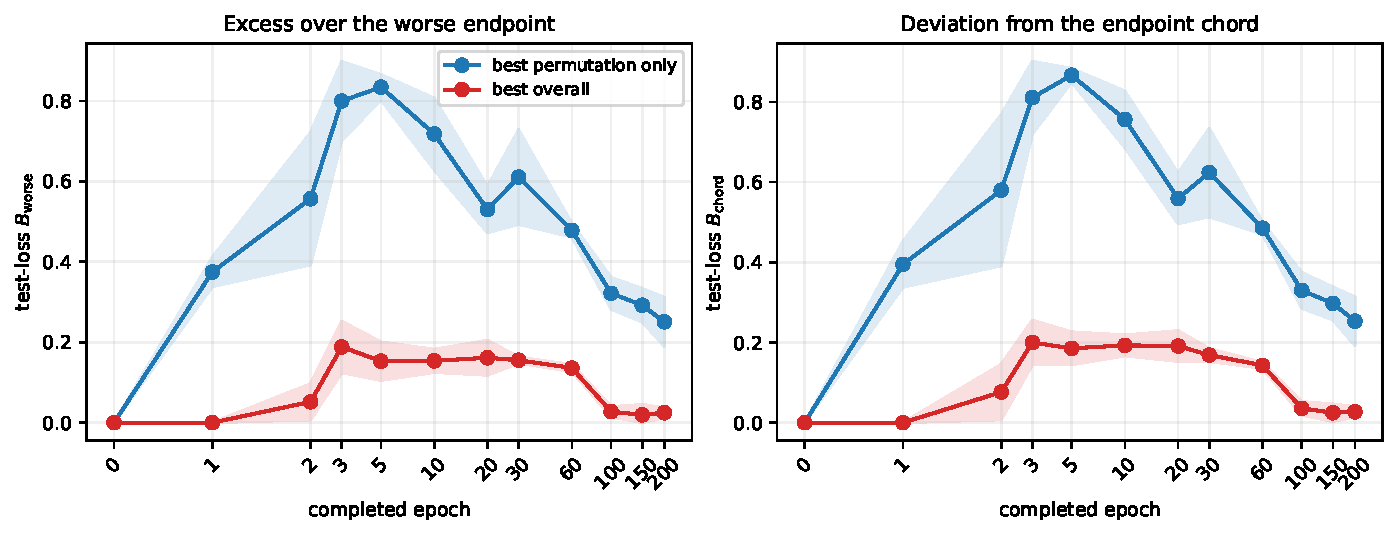
\includegraphics[width=\linewidth]{linear_stage_summary.pdf}
    \caption{Same-stage linear connectivity.  Both panels report test loss;
    the left uses $\Bworse$ and the right uses $\Bchord$.  Curves show mean
    $\pm$ one standard deviation across three seed pairs.}
    \label{fig:linear-same}
\end{figure}

Positive scaling produces the main improvement.  The best overall
$\Bworse$ is zero through epoch 1, rises to $0.188$ at epoch 3, stays near
$0.14$--$0.16$ through epoch 60, and falls to $0.025$ at epoch 200.  Every
validation-selected overall method is scale-aware: Sinkhorn plus scale
refinement is selected for 91 of 144 ordered cells, WM plus scale for 52, and
joint Sinkhorn plus scale once.  Among permutation-only methods, Sinkhorn wins
86 cells and WM 58.

\begin{table}[H]
\centering
\small
\caption{Selected same-stage test-loss barriers, mean $\pm$ standard deviation
over three seed pairs.}
\label{tab:linear}
\begin{tabular}{rccc}
\toprule
Epoch & Permutation-only $\Bworse$ & Overall $\Bworse$ & Overall $\Bchord$ \\
\midrule
0   & $0.000\pm0.000$ & $0.000\pm0.000$ & $0.000\pm0.000$ \\
1   & $0.375\pm0.037$ & $0.000\pm0.000$ & $0.000\pm0.000$ \\
3   & $0.800\pm0.099$ & $0.188\pm0.064$ & $0.200\pm0.056$ \\
5   & $0.834\pm0.032$ & $0.153\pm0.048$ & $0.185\pm0.041$ \\
60  & $0.478\pm0.017$ & $0.136\pm0.009$ & $0.143\pm0.007$ \\
100 & $0.322\pm0.039$ & $0.027\pm0.012$ & $0.036\pm0.017$ \\
200 & $0.251\pm0.061$ & $0.025\pm0.012$ & $0.027\pm0.012$ \\
\bottomrule
\end{tabular}
\end{table}

Across the complete checkpoint matrix, the mean test-loss $\Bworse$ falls
from $0.431$ with the best permutation-only alignment to $0.0408$ with the best
overall method, a $90.5\%$ reduction.  Mean test-error $\Bworse$ similarly
falls from $15.31$ to $1.48$ percentage points.  Positive scaling therefore
explains a large part of the mismatch left by permutation.

\subsection{Cross-stage results}

Figure~\ref{fig:linear-cross} shows final/intermediate pairs.  For
$n\in\{0,1\}$, $\Bworse$ is zero in both directions, but $\Bchord$ remains
between $0.30$ and $0.70$.  The early endpoint provides such a high baseline
that the interpolation does not exceed it, even though the path rises well
above the endpoint chord.  By epochs 60--200, the two definitions and both
directions are much closer.

\begin{figure}[H]
    \centering
    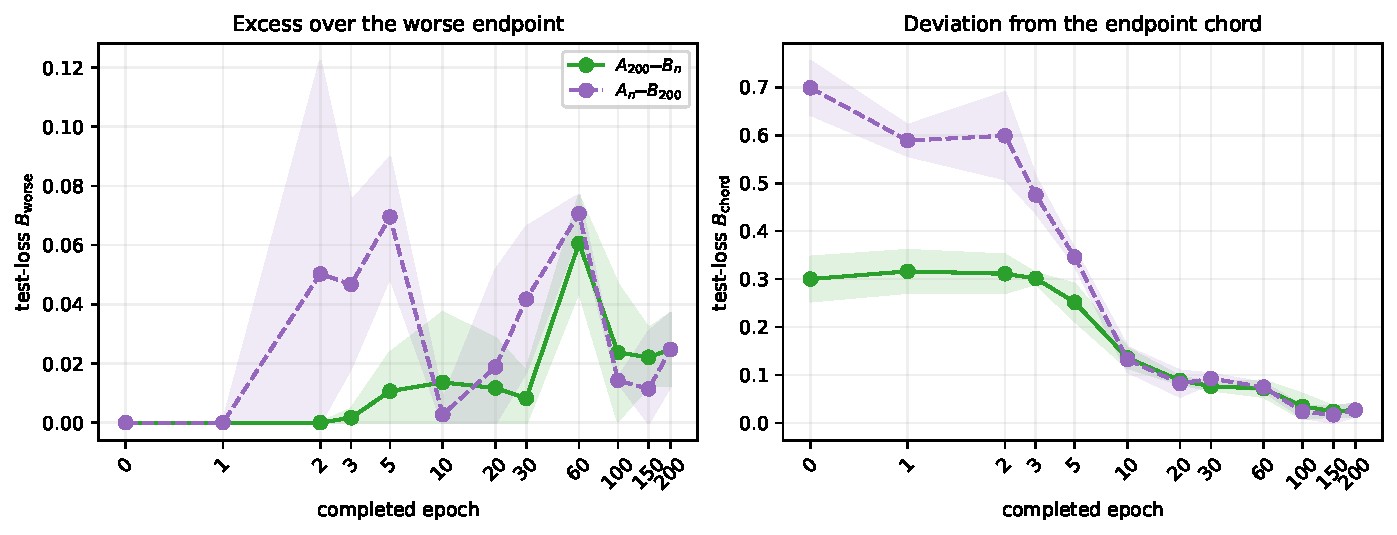
\includegraphics[width=\linewidth]{linear_cross_stage.pdf}
    \caption{Cross-stage linear connectivity after the best overall alignment.
    Both panels report test loss and show mean $\pm$ one standard deviation
    over three seed pairs.}
    \label{fig:linear-cross}
\end{figure}

The cross-stage result is the clearest reason not to report only one barrier
definition.  A statement that early/final pairs have ``zero barrier'' is true
under $\Bworse$ but incomplete under $\Bchord$.

\section{Nonlinear stage connectivity}

The nonlinear experiment contains 168 primary paths across the three seed
pairs.  Figure~\ref{fig:nonlinear} compares raw linear interpolation with the
validation-selected curved path.  For independent same-stage models, the mean
raw test-loss $\Bchord$ is $1.495$, while the selected nonlinear mean is
$0.0029$, a $99.8\%$ reduction.  The corresponding reductions are $99.6\%$ for
$A_{200}$--$B_n$ and $99.4\%$ for $A_n$--$B_{200}$.

\begin{figure}[H]
    \centering
    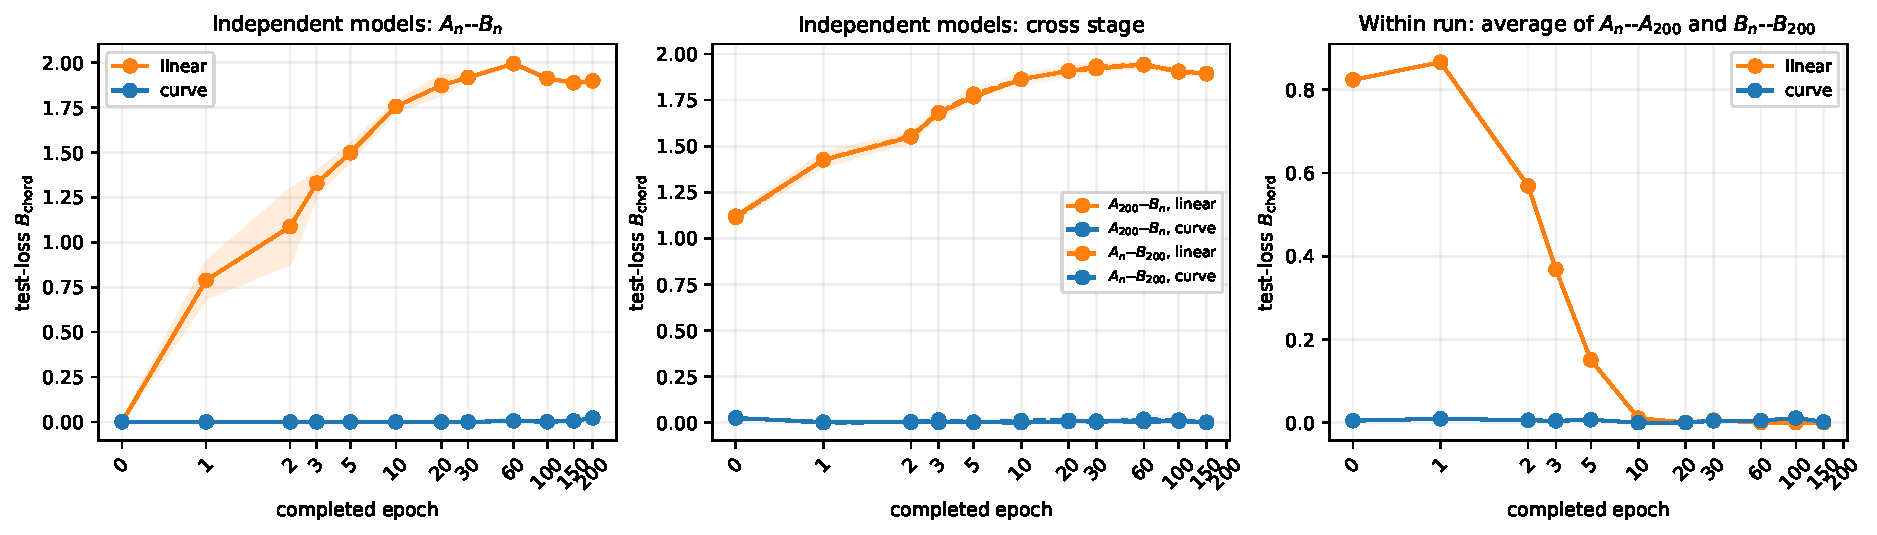
\includegraphics[width=\linewidth]{nonlinear_stage_summary.pdf}
    \caption{Test-loss $\Bchord$ for raw linear interpolation and optimized
    nonlinear paths.  The panels separate same-stage independent models,
    cross-stage independent models, and within-run controls.}
    \label{fig:nonlinear}
\end{figure}

\begin{table}[H]
\centering
\small
\caption{Aggregate test-loss $\Bchord$ for raw linear and selected nonlinear
paths.}
\label{tab:nonlinear}
\begin{tabular}{lrrr}
\toprule
Path group & Paths & Linear mean & Nonlinear mean \\
\midrule
Same stage & 36 & 1.495 & 0.0029 \\
$A_{200}$--$B_n$ & 33 & 1.725 & 0.0065 \\
$A_n$--$B_{200}$ & 33 & 1.727 & 0.0099 \\
Within A & 33 & 0.256 & 0.0053 \\
Within B & 33 & 0.253 & 0.0047 \\
\bottomrule
\end{tabular}
\end{table}

All 168 selected paths have sampled test-loss $\Bchord\leq0.05$, and 150 are
below 0.02.  Error is less uniformly controlled: 121 paths satisfy both loss
$\Bchord\leq0.02$ and error $\Bchord\leq1.5$ percentage points.  For the three
final--final pairs, mean test-loss $\Bchord$ is $0.022\pm0.020$, while mean
test-error $\Bchord$ is $2.16\pm1.95$ points.

The within-run control follows a different pattern.  Raw interpolation from an
early checkpoint to epoch 200 has a barrier, but paths starting around epoch 10
are already close to linearly connected.  Late SGD checkpoints therefore stay
in a locally compatible region even though independently trained models remain
incompatible without alignment or curvature.

\section{Conclusions and qualifications}

The current results support four conclusions:

\begin{enumerate}
    \item Linear incompatibility between independent VGG11 runs appears within
    the first few epochs and later decreases; it does not grow monotonically.
    \item Permutation alignment explains only part of this incompatibility.
    Positive ReLU scaling removes about 90\% of the remaining mean test-loss
    $\Bworse$ across the checkpoint matrix.
    \item $\Bchord$ and $\Bworse$ give materially different accounts of early
    cross-stage pairs, so both should be reported.
    \item Optimized B\'ezier and polygonal paths avoid almost all of the raw
    linear test-loss barrier for the tested checkpoint pairs.
\end{enumerate}

Three qualifications matter.  First, the linear results use the full test set,
whereas the current nonlinear profiles use a fixed 2,000-example test subset;
the nonlinear selections should be re-evaluated on the full test set before a
single direct comparison figure is used in the paper.  Second, the original
nonlinear final--final pilot gate was not met because its error threshold had
been inherited from a VGG16 experiment; proceeding with the VGG11 paths was an
explicitly recorded decision.  Third, a found path is evidence of connectivity
for the sampled data and grid, while a failed search would not prove that no
path exists.

The next useful step is evaluation-only: keep all selected nonlinear paths
fixed and evaluate them on the same data used by the linear report.  No path
refitting is required.

\section*{Artifacts}

The report uses:
\begin{itemize}
    \item \path{results/dense_linear_stage_vgg11_10k/};
    \item \path{results/nonlinear_stage_vgg11_fullfit/}.
\end{itemize}
Its figures can be regenerated with \texttt{make\_figures.py} in this directory.

\clearpage
\section*{Appendix: Absolute profiles for all ordered stage pairs}

The following pages reproduce the complete absolute interpolation profiles for
all ordered VGG11 checkpoint pairs from the dense linear-stage experiment.

\includepdf[
    pages=-,
    pagecommand={\thispagestyle{plain}}
]{../../results/dense_linear_stage_vgg11_10k/report/absolute_profiles_all_stage_pairs.pdf}

\end{document}
